

\section{Architecture Logiciel}

Nous avons divisé notre modèle en deux grandes architectures, le serveur et les unités. 

\subsection{Architecture du serveur}



\subsection{Architecture des unités}

\begin{figure}[H]
    \centering
    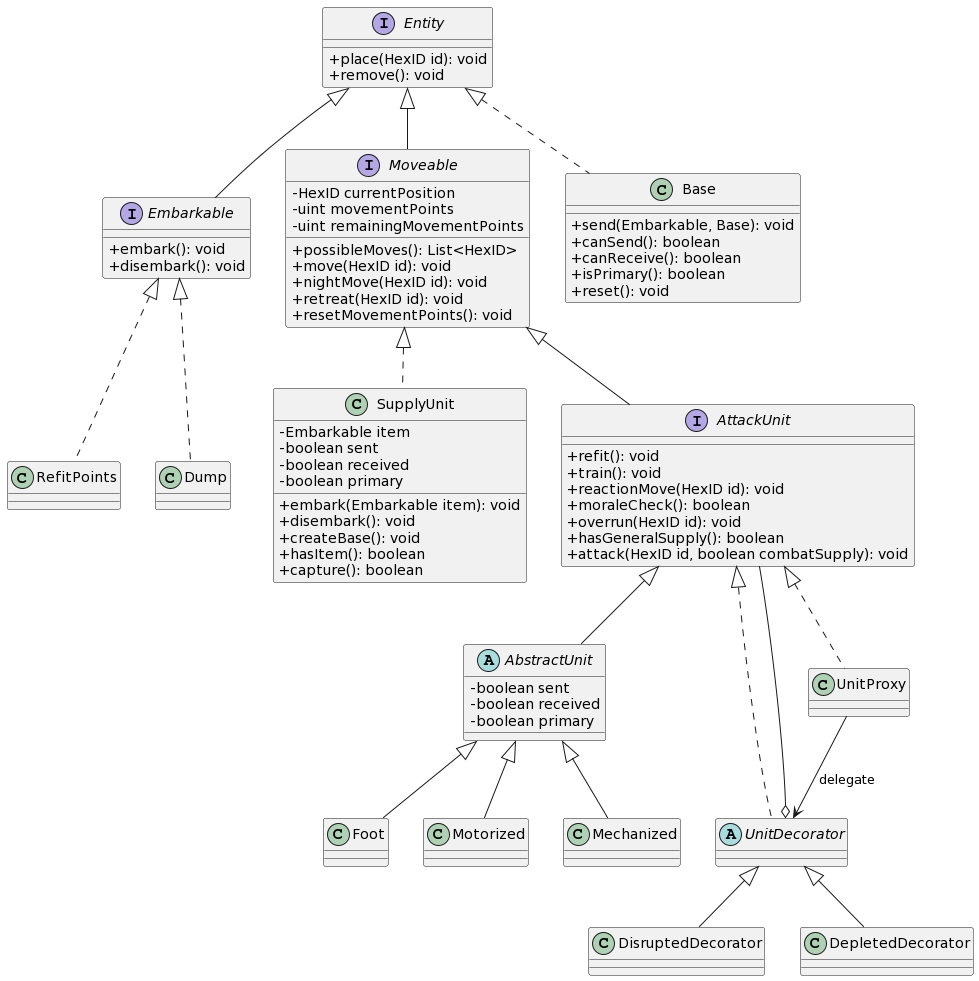
\includegraphics[scale=0.3]{data/uml_entityV4.png}
    \caption{Diagramme UML de l'objet \emph{Entity}}
    \label{fig:uml_entity}
\end{figure}

Nous avons fait le choix de réunir toutes les unités sous la même interface, ce qui nous permet d'avoir un seul type pour toutes les unités et donc de pouvoir faire des listes de ces entités dans la partie serveur.
Pour une meilleure factorisation on sépare les unités en deux, celles qui peuvent bouger (\lstinline{Moveable}) et les autres. Nous séparons de nouveau en unités de soutien et d'attaque. Pour assurer la maintenance du code et rajouter des fonctionnalités, nous avons utilisé deux designs patterns, le \lstinline{Decorator} et le \lstinline{Proxy}. Mais pour pouvoir utiliser ces patterns nous avions la contrainte suivante, il fallait que les deux patterns implémentent une interface comme montrer ci-dessous. Nous avons donc était forcé d'ajouter une interface intermédiaire (ici \lstinline{AttackUnit}) pour pouvoir les implémenter. Le décorateur nous permet de changer le comportement des unités dynamiquement sans à avoir à changer toutes les classes qui étendent \lstinline{AbstractUnit}. Mais l'utilisation de ce pattern conduit à un problème, on peut appliquer un décorateur à un objet déjà décorer un nombre de fois infinie. Ce qui nous amène donc à utiliser un \lstinline{Proxy} qui permet de contrôler l'utilisation du décorateur. 

Toute la démonstration précédente était notre réflexion lors de la conception de l'architecture. Mais nous avons implémenté l'attaque en dernier, il est donc possible que les patterns énoncés ne soient pas présents dans le code.

\begin{figure}[H]
    \centering
    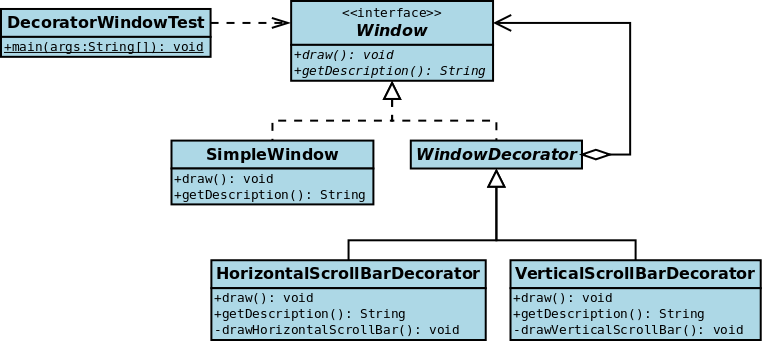
\includegraphics[scale=0.3]{data/UML_Decorator_Pattern_Exmple.png}
    \caption{Exemple Wikipedia à rajouter dans bibliographie}
\end{figure}

\begin{figure}[H]
    \centering
    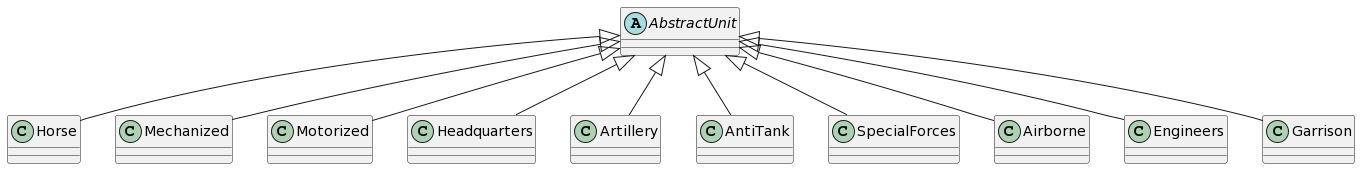
\includegraphics[scale=0.3]{data/uml_abstract_unit.png}
    \caption{Diagramme UML des unités}
\end{figure}

Dans les règles ils existent toutes les unités d'attaque qui se trouvent ci-dessus. Comme nous avions un temps limité nous avons décidé de ne pas toutes les implémenter car même si certaines ont un comportement différent le travail aurait été chronophage et donc nous avons privilégié des aspects plus importants du projet. On peut trouver les unités d'attaque choisies dans le diagramme \ref{fig:uml_entity} (Foot, Mechanized, Motorized).

\section{Technologies}

\subsection{Service d'hébergement}

Pour le service d'hébergement nous avons utilisé le GitLab du Cremi comme demandé dans les consignes. Nous avons paramétré les pipelines pour qu'à chaques commits il effectue les tests automatiquement pour aider à ne pas faire des commits complètement erronés. Concernant les branches nous avons divisé le dépôt en quatre:
\begin{itemize}
    \item main
    \item dev
    \item backend
    \item frontend
\end{itemize}

Le principe est que l'on développe sur les branches correspondantes (\lstinline{frontend} et \lstinline{backend}), que l'on fusionne ces deux dernières sur la branche \lstinline{dev} pour vérifier si tout se passe bien et enfin mettre à jour le main pour avoir une version stable. Cela nous paraissait le plus logique sauf que l'on s'est vite rendu compte que ce n'était pas le moyen le plus optimisé de travailler car lorsqu'on travaille sur la même chose sur le \lstinline{backend} et le \lstinline{frontend} cela produisait divers bugs lorsqu'on réunissait les deux branches. Il aurait sûrement plutôt réfléchir en features et donc créer une branche pour chaque tâche.

\subsection{Langage de programmation}

Nous avons choisi comme langage de programmation \lstinline{TypeScript} pour le \lstinline{backend} et le \lstinline{frontend}. En effet en ayant la même technologie pour tout le projet cela rend la communication beaucoup plus simple entre les deux côtés. On aurait aussi pu utiliser \lstinline{JavaScript} mais une surcouche de typage nous permet de sécuriser la production du code. Enfin ce choix nous a laissé la liberté de ne pas faire que de la programmation objet, par exemple le \lstinline{frontend} est en majorité de la programmation impérative.

\subsection{Communication client-serveur}

Au départ nous étions parti sur une architecture avec un serveur web qui communiquait avec les clients grâce à des requêtes web HTTP.

Malheureusement cette architecture n'était pas adaptée pour un jeu de ce type puisque au moment où un joueur joue un coup, l'autre joueur doit être notifié de ce changement. Or si on utilise un serveur web HTTP le client devrait faire une requête au serveur pour être mis au courant, ce qui n'est pas pratique.

Pour un changement en direct sans faire une boucle de requêtes continuelles, il faudrait un système où le serveur peut envoyer un message au client sans requête au préalable.

C'est pour cela qu'une architecture avec des web sockets a été la solution que nous avons choisie.
Cette architecture permet d'envoyer des messages ou des données aux clients sans requête préalable.


\begin{figure}[H]
    \centering
    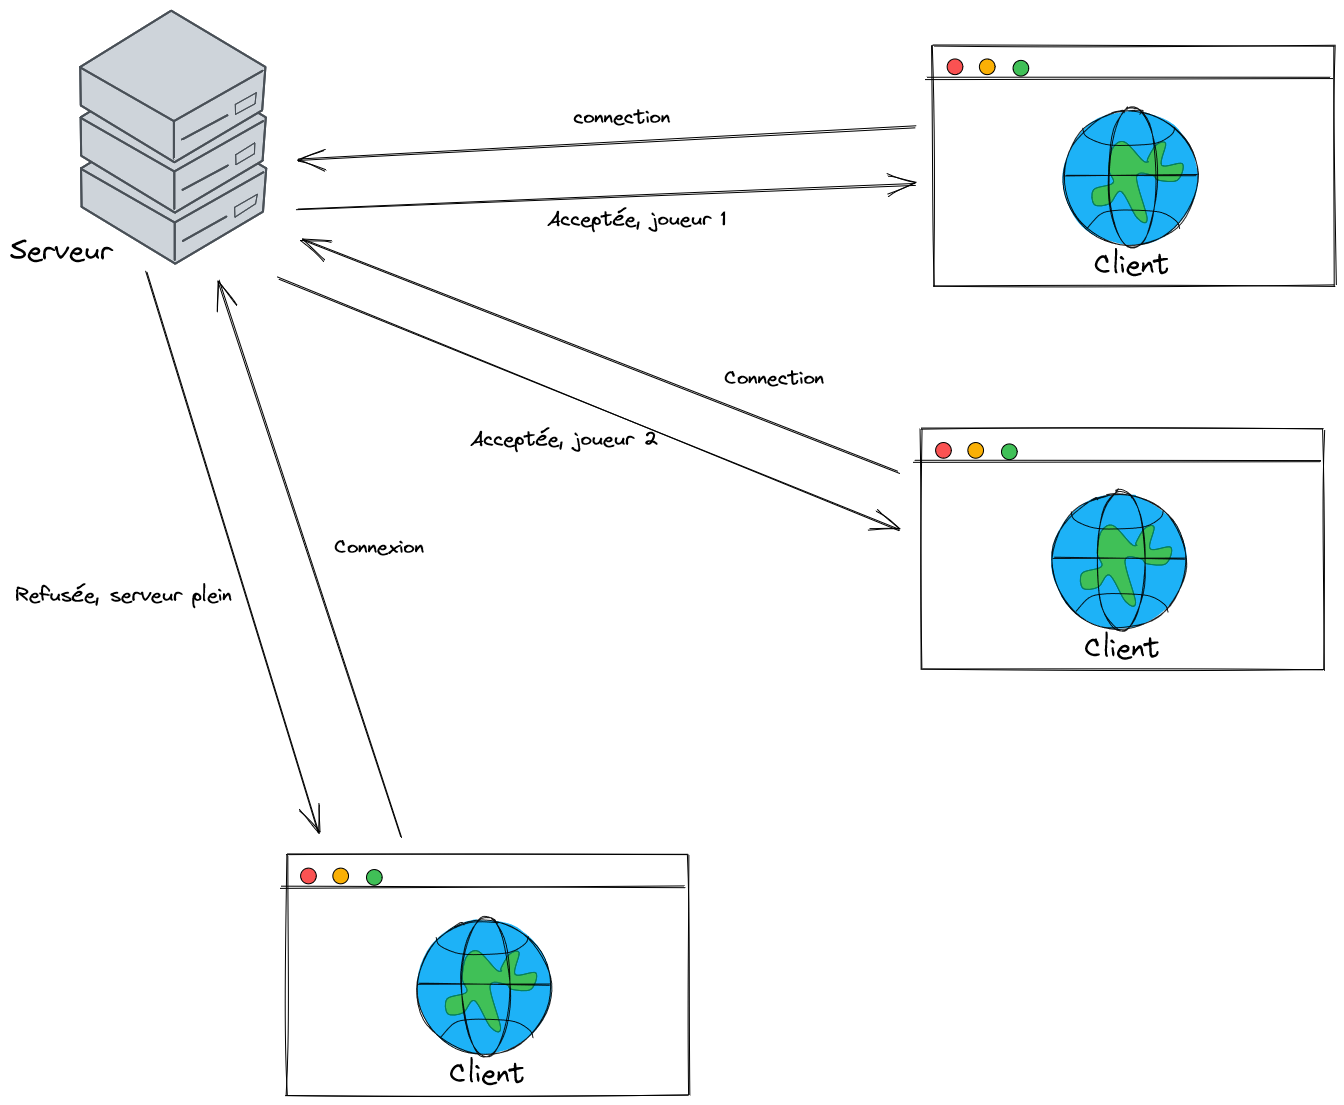
\includegraphics[scale=0.25]{data/reseau_initialisation.png}
    \caption{Phase de connexion des joueurs au serveur}
\end{figure}

Ici on peut voir la première phase du serveur qui permet d'enregistrer les connexions des deux joueurs pour créer une partie.

La partie de connexion est gérée par la bibliothèque {\tt socket-io} que nous utilisons pour le serveur et le client. C'est l'avantage essentiel d'utiliser la même technologie sur le backend et le frontend.

Dans le serveur, nous sauvegardons les sockets qui se connectent au serveur. La limite est de 2 puisqu'il y a 2 joueurs maximum. Quand les 2 joueurs sont bien connectés, la partie est pleine. S'il y en a déjà 2 lors d'une connexion d'un troisième socket, alors la connexion de la troisième est refusée et cette dernière reçoit un code d'erreur, {\tt full}, que le frontend de ce socket va afficher à l'utilisateur.
Si un autre joueur essaie de se connecter, alors le socket n'est pas sauvegardé dans le serveur et elle est déconnectée, il reçoit également une erreur, {\tt full}, qui va s'afficher dans le terminal.

Une fois les deux joueurs créés et la partie initialisée, la carte est envoyée aux deux joueurs pour l'affichage. Voir ci-dessous \ref{reseau_carte}.

\begin{figure}[H]
    \centering
    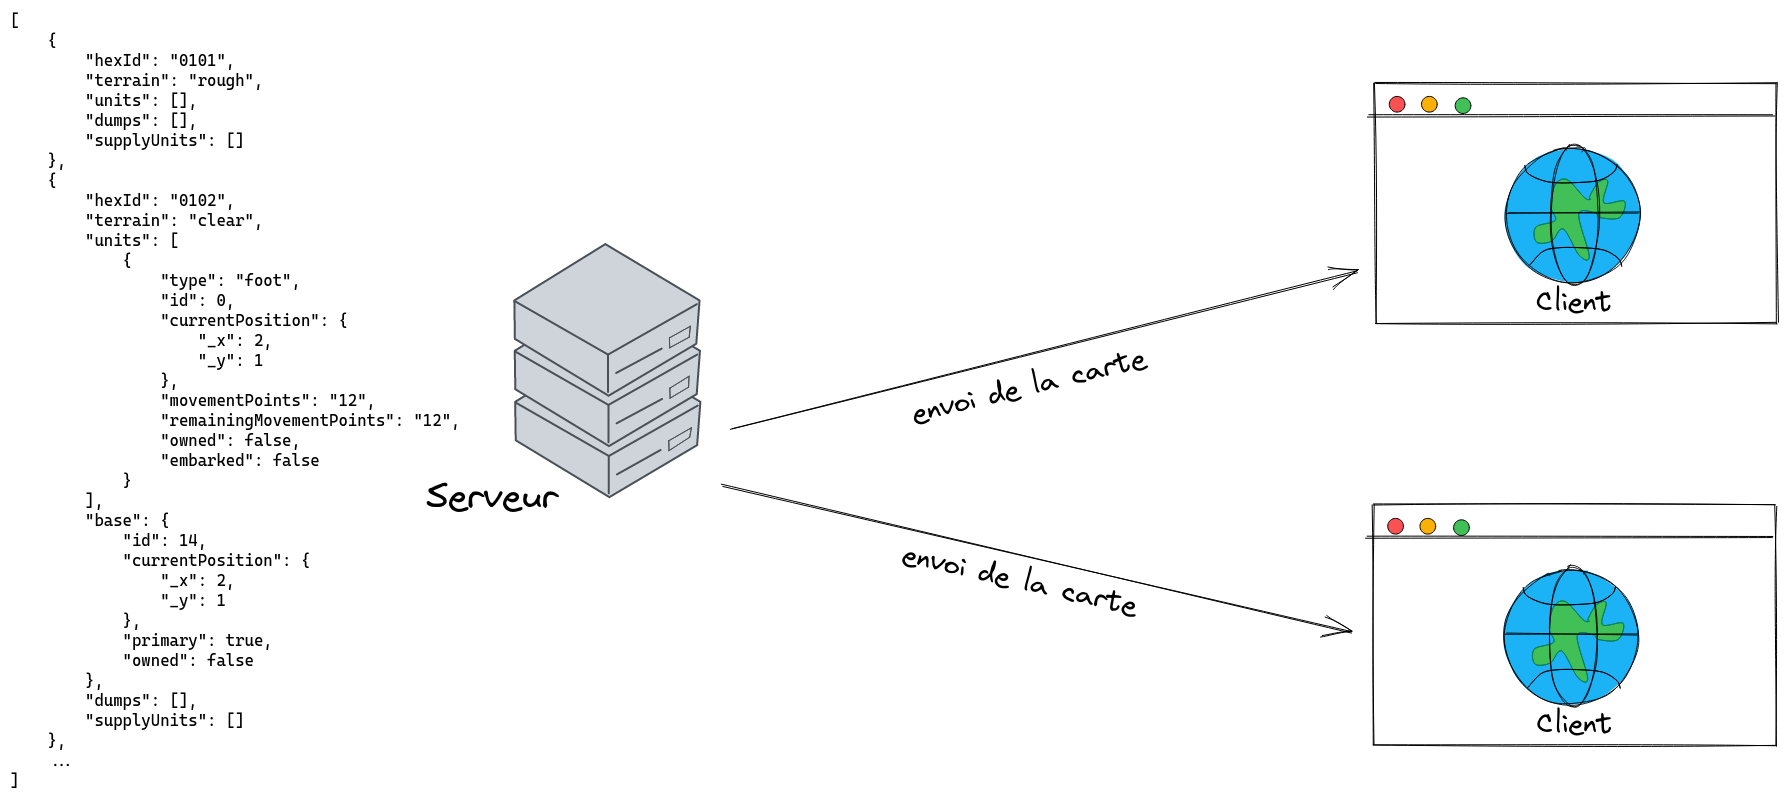
\includegraphics[scale=0.25]{data/reseau_map.png}
    \caption{Phase de connexion des joueurs au serveur}
    \label{reseau_carte}
\end{figure}

Le code à gauche du serveur est le début du {\tt JSON} original envoyé à chaque client.
On peut voir comment il est constitué : c'est un tableau d'objets. Chacun de ces objets représente une case.
Chaque case possède un ``id``, un identifiant, ainsi qu'un ``terrain`` qui décrit son type de terrain.
Il possède aussi 3 aux champs, ``units``, ``dumps`` et ``supplyUnits`` qui sont des tableaux d'objets.
Comme leurs noms l'indique ces objets représentent des tableaux d'unités, de dépôts ou d'unités de ravitaillement.

À partir de ce moment-là, le moteur graphique du jeu est chargé de dessiner la carte reçue en JSON.
L'action \ref{reseau_carte} se répète à chaque changement de la carte dans le jeu.


Les phases vont donc s'enchaîner jusqu'à ce qu'une action d'un joueur soit requise.

\begin{figure}[H]
    \centering
    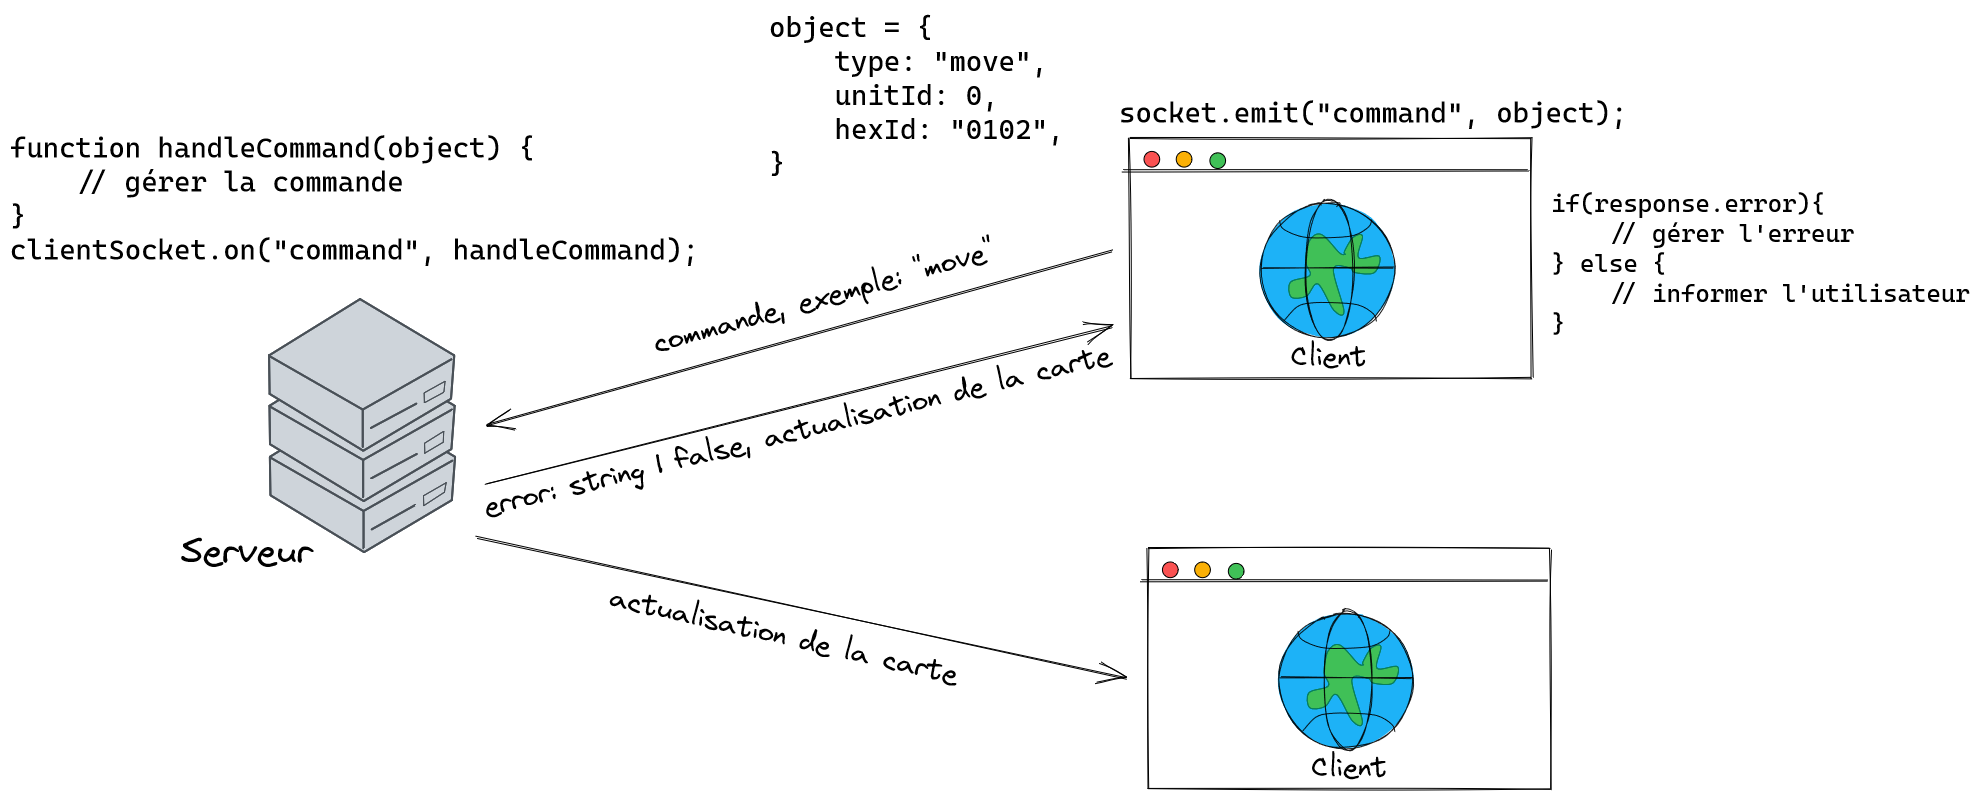
\includegraphics[scale=0.25]{data/reseau_commande.png}
    \caption{Phase de jeu, exemple de commande {\tt move}}
\end{figure}

TODO

La partie s'exécute normalement jusqu'à la fin.

\subsection{}

Vue.js

\subsection{Test}

Pour les tests nous avons utilisé Mocha qui est un cadre de test JavaScript pour les programmes Node.js. Nous testons le backend et les communications des sockets parce qu'il est compliqué de tester l'affichage. Nous avons réalisé des tests unitaires, la couverture du code est aussi vérifiée grâce à NYC qui est un framework compatible avec Mocha. Nous y reviendrons plus tard dans une partie dédiée.

\subsection{Interface graphique}

Dans le sujet il était indiqué que l'on n'était pas dans l'obligation de faire une interface graphique. Mais afficher un hexagone dans un terminal est compliqué et la moitié de la carte donnée en exemple est de dimensions 32*29 cases, ce qui aurait donné un rendu illisible. Nous avons donc fait le choix de faire une interface graphique. Pour afficher la carte nous avons testé plusieurs bibliothèques et choisis \lstinline{P5.js} pour plusieurs raisons, la documentation est claire et la bibliothèque est plutôt populaire ce qui facilite les recherches lors de problèmes d'implantation (tutoriels, stackoverflow...).

Notre approche pour afficher la carte est de la dessiner à chaque changement dans le \lstinline{backend} (exemple: un move). La première raison à cette tactique est de rendre l'affichage plus facile vu que ce n'est pas la priorité du sujet. Et si nous avions dû faire un affichage dynamique il aurait fallu créer des objets pour sauvegarder la position des unités dans chaque case. Ce qui implique aussi une duplication de la logique du \lstinline{backend}, nous avons voulu éviter ça. Ici le \lstinline{backend} envoie des données, on les parse et on les affiche.

Pour dessiner les hexagones de la map nous avons cherché des algorithmes pour ne pas avoir à les développer nous-mêmes mais nous n'avons trouvé que des affichages comme suivant.

\begin{figure}[H]
    \centering
    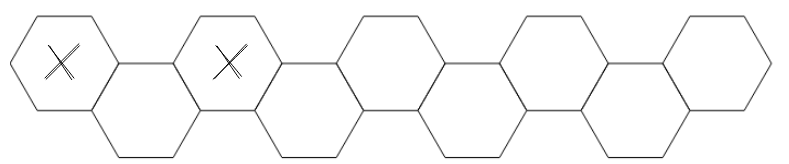
\includegraphics[scale=0.3]{data/hexmap_exemple.png}
    \caption{Une ligne d'hexagones}
\end{figure}
% source https://eperezcosano.github.io/hex-grid

 Le problème de ce genre d'affichage est que deux cases sur la même ligne (avec les croix) ne se touchent pas. On ne peut donc pas faire de déplacement d'unité. Nous avons alors fait nos propres méthodes pour avoir un hexagone dans l'autre sens (avec la pointe vers le haut) et qui est donc adjacente à ses six voisins comme suit. Pour cela on calcule les points grâce au cercle trigonométrique.
 
\begin{figure}[H]
    \centering
    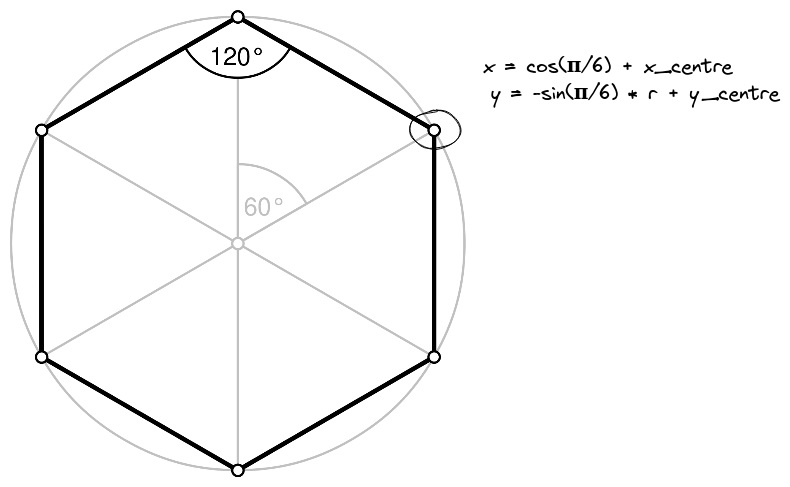
\includegraphics[scale=0.3]{data/hexagon.png}
    \caption{Les étapes pour dessiner un hexagone}
\end{figure}

 On peut aussi mettre six unités d'attaque dans une case, on réutilise donc le calcul de ces points pour faire la moyenne par rapport au centre. On se retrouve donc avec une unité dans chaque coin de l'hexagone. Ce qui donne le résultat suivant.
 
\begin{figure}[H]
    \centering
    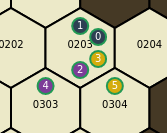
\includegraphics[scale=.7]{data/hexagon_with_units.png}
    \caption{Affichage hexagone avec des unités}
\end{figure}

